\graphicspath{{./figures/capitolo7/}}
\lstset{inputpath = ./programs/capitolo7}
\pgfplotstableset{search path = ./tables/capitolo7}

\chapter{Dai punti di equilibrio agli strani attrattori}

Nel capitolo precedente ci siamo concentrati esclusivamente su strutture
di equilibrio \emph{puntuali}; in questo capitolo vedremo invece alcuni esempi
di \emph{insiemi} di equilibrio, sia attrattivi sia invarianti, che lasciano
intuire quanto possano essere ricche, complesse e addirittura caotiche le dinamiche
nonlineari di un sistema dinamico continuo o discreto. Vista la difficoltà
di un approccio teorico all'argomento, ci limiteremo alla sola sperimentazione
numerica, con lo scopo di visualizzare queste strutture (nei limiti del possibile).

\section{Modello preda-predatore}

Il \emph{modello preda-predatore}, noto anche come \emph{modello di Lotka-Volterra},
è un modello matematico molto versatile, che nella sua formulazione classica
descrive la dinamica del numero di individui $x(t)$ e $y(t)$ appartenenti
a due popolazioni animali distinte: la prima popolazione è quella delle
\emph{prede}, che in assenza di predatori crescerebbe esponenzialmente ma
è frenata da un tasso di predazione proporzionale a $x(t)y(t)$, mentre la
seconda è quella dei \emph{predatori}, che in assenza di prede decrescerebbe
esponenzialmente ma è sostenuta dallo stesso tasso di predazione $x(t)y(t)$
(anche se la costante di proporzionalità è solitamente inferiore a quella delle prede).
Il matematico italiano Vito Volterra riuscì a spiegare con questo modello
un fenomeno controintuitivo osservato nella fauna del mare Adriatico
durante la prima guerra mondiale: la riduzione dell'attività di pesca
dovuta al conflitto provocò una diminuzione in media del rapporto tra
prede e predatori, nonostante tale attività interessasse in misura uguale
entrambe le popolazioni.

Formalmente, il modello è definito dal seguente sistema di equazioni differenziali:
\begin{equation} \label{eq:modello-preda-predatore}
\left\{
\begin{aligned}
x'(t) &=  ax(t) -bx(t)y(t) \\
y'(t) &= -cx(t) +dx(t)y(t)
\end{aligned}
\right.
\end{equation}
I segni dei coefficienti sono stati scelti in modo che $a,b,c,d$ siano tutte costanti
positive. In ordine, tali costanti sono dette \emph{tasso di riproduzione
delle prede}, \emph{tasso di predazione che riduce le prede}, \emph{tasso di
mortalità dei predatori} e \emph{tasso di predazione che aumenta i predatori}.
Si verifica facilmente che il sistema \eqref{eq:modello-preda-predatore} ha due
punti di equilibrio: l'origine $(0,0)$ e il punto $(x^*,y^*)$ definito da
\[
x^* = \frac{c}{d}, \quad y^* = \frac{a}{b}.
\]
Linearizzando il sistema \eqref{eq:modello-preda-predatore} intorno ai due punti
di equilibrio si trova che l'origine è un punto di equilibrio instabile
(Teorema \ref{teor:linearizzazione-instabilità}),
mentre non si può dire nulla del punto $(x^*,y^*)$
perché si ottiene una matrice con autovalori distinti e puramente immaginari.
È possibile però ricostruire l'andamento delle traiettorie eliminando il
tempo $t$ dal sistema \eqref{eq:modello-preda-predatore} e ottenendo così
un'equazione implicita nelle variabili $x$ e $y$ che vincola il moto
nel piano delle fasi:
\[
\eta(x)^c \, \xi(y)^a = K, \quad \text{con $\eta(x) = xe^{-x/x^*}\!\!$,
$\,\xi(y) = ye^{-y/y^*}\!\!$, $\,K>0$.}
\]
A partire da questa osservazione, ulteriori considerazioni qualitative 
permettono di dimostrare che le popolazioni $x(t)$ e $y(t)$ sono funzioni
periodiche del tempo, con lo stesso periodo $T$. Naturalmente, sia $K$ che $T$
dipendono dalle condizioni iniziali $x(0) = x_0$ e $y(0) = y_0$.
Gli insiemi di equilibrio invarianti per l'equazione di Lotka-Volterra
sul piano $(\eta,\xi)$ sono dunque delle curve chiuse formate da rami
di iperboli generalizzate (cioè, non necessariamente quadriche).

Dato che il rapporto tra prede e predatori è una funzione periodica del tempo,
il fenomeno riguardante la fauna adriatica andrà spiegato non in termini
delle quantità istantanee $x(t)$ e $y(t)$, bensì in termini delle
quantità medie
\[
\bar{x} = \int_0^T x(t) \dt \quad \text{e} \quad \bar{y} = \int_0^T y(t) \dt.
\]
Un'opportuna sostituzione delle equazioni del sistema \eqref{eq:modello-preda-predatore}
all'interno di questi integrali permette di dimostrare che
$\bar{x} = x^* = c/d$ e che $\bar{y} = y^* = a/b$.
Dunque, il punto di equilibrio $(x^*,y^*)$ in questo modello può essere
interpretato come il valore medio delle due popolazioni durante ogni periodo
della dinamica (e, quindi, anche il valore medio su tempi lunghi).

Indichiamo con $r$ il rapporto tra il numero medio di prede $\bar{x}$ e il
numero medio di predatori $\bar{y}$. Se si suppone che la riduzione dell'attività
di pesca durante la prima guerra mondiale si possa modellare con un termine aggiuntivo
$(-\varepsilon x(t), -\varepsilon y(t))$ al sistema \eqref{eq:modello-preda-predatore},
la dinamica delle popolazioni sarà descritta dal nuovo sistema
\begin{equation} \label{eq:modello-preda-predatore-epsilon}
\left\{
\begin{aligned}
x'(t) &=  (a-\varepsilon)x(t) -bx(t)y(t) \\
y'(t) &= -(c+\varepsilon)x(t) +dx(t)y(t)
\end{aligned}
\right.
\end{equation}
e il rapporto tra i valori medi sarà funzione di $\varepsilon$:
\[
r(\varepsilon) = \frac{c+\varepsilon}{d} \frac{b}{a-\varepsilon}.
\]
Il motivo della riduzione del rapporto $r = \bar{x}/\bar{y}$  al diminuire
dell'attività di pesca è pertanto spiegato dal fatto che $r(\epsilon)$ sia
una funzione crescente di $\varepsilon$.
A conferma di questa analisi qualitativa del modello, abbiamo scritto il
Programma \ref{prog:lotka-volterra}, che effettua una simulazione della
dinamica con parametri
\[
a = 2, \quad
b = 0.04, \quad
c = 1, \quad
d = 0.001, \quad
t \in [0,40], \quad
x(0) = 800, \quad
y(0) = 60.
\]

\lstinputlisting[float=!bp, label=prog:lotka-volterra, linerange={1-16},
caption={Simulazione del modello preda-predatore.}]{lotka_volterra.m}

\noindent In questo esempio si ha che $\bar{x} = c/d = 1000$ e $\bar{y} = a/b = 50$,
quindi le oscillazioni della popolazione sono dovute a un iniziale difetto
di prede ed eccesso di predatori. Si può dimostrare che la simulazione
copre nove periodi, perché il periodo $T$ del moto è circa 4.5.
Durante la simulazione, il tasso di pesca $\varepsilon$ viene fatto variare
secondo la legge
\[
\epsilon(t) = -\frac{0.2}{1+e^{-t+20}}.
\]
Questa legge (una \emph{sigmoide}) è stata scelta in modo da passare gradualmente
da $\varepsilon = 0$ a $\varepsilon = -0.2$ in un intorno di $t = 20$,
simulando così la riduzione dell'attività di pesca nella seconda metà
della simulazione. Nella Figura \ref{fig:lotka-volterra-rapporto}
si può vedere come la riduzione di $\varepsilon$ sposti in basso
l'asse attorno al quale avvengono le oscillazioni del rapporto $x(t)/y(t)$,
in accordo con la teoria.
Per completezza riportiamo anche le Figure \ref{fig:lotka-volterra-popolazioni}
e \ref{fig:lotka-volterra-piano-delle-fasi}, in cui si può vedere l'andamento
delle popolazioni in funzione del tempo e lo spostamento da un insieme
di equilibrio relativo a $\varepsilon = 0$ con centro $(1000,50)$ a un altro
insieme di equilibrio relativo a $\varepsilon = -0.2$ con centro $(800,55)$.

\begin{figure}[tbp]
\centering
\begin{tikzpicture}[trim axis left, trim axis right]
\begin{axis}[
	scale only axis,
	xlabel={$t$},
	ylabel={$x(t)/y(t)$},
	width=0.8\textwidth,
	height=0.4\textwidth,
]
\addplot[black] table[x=t, y=ratio] {lotka-volterra.dat};
\addplot[dashed, domain= 0:20] expression {20};
\addplot[dashed, domain=20:40] expression {14.5};
\end{axis}
\end{tikzpicture}
\caption{Rapporto tra prede e predatori in funzione del tempo.}
\label{fig:lotka-volterra-rapporto}
\end{figure}

\begin{figure}[tbp]
\centering
\begin{tikzpicture}[trim axis left, trim axis right]
\pgfplotsset{
	set layers,
	y axis style/.style={
        yticklabel style=#1,
        ylabel style=#1,
        y axis line style=#1,
        ytick style=#1,
   }
}
\begin{axis}[
	scale only axis,
	xmin=-4,
	xmax=44,
	axis y line*=left,
	xlabel=$t$,
	ylabel={$x(t)$},
	y axis style=blue!75!black,
	width=0.8\textwidth,
	height=0.4\textwidth,
]
\addplot[blue] table[x=t, y=y1] {lotka-volterra.dat}; \label{pgfplots:plot1}
\end{axis}
\begin{axis}[
	scale only axis,
	xmin=-4,
	xmax=44,
	axis y line*=right,
	axis x line=none,
	ylabel={$y(t)$},
	y axis style=red!75!black,
	width=0.8\textwidth,
	height=0.4\textwidth,
]
\addplot[red] table[x=t, y=y2] {lotka-volterra.dat}; \label{pgfplots:plot2}
\end{axis}
\end{tikzpicture}
\caption{Numero di prede (in blu) e predatori (in rosso) in funzione del tempo.}
\label{fig:lotka-volterra-popolazioni}
\end{figure}

\begin{figure}[tbp]
\centering
\begin{tikzpicture}[trim axis left, trim axis right]
\begin{axis}[
	xlabel={Prede $x$},
	ylabel={Predatori $y$},
	width=0.9\textwidth,
	height=0.7\textwidth,
]
\addplot[black] table[x=y1, y=y2] {lotka-volterra.dat};
\addplot[black, only marks, mark=+, mark size=0.4em, line width=0.1em] coordinates{(1000,50)};
\addplot[black, only marks, mark=+, mark size=0.4em, line width=0.1em] coordinates{(800,55)};
\end{axis}
\end{tikzpicture}
\caption{Dinamica delle popolazioni di prede e predatori nel piano delle fasi.}
\label{fig:lotka-volterra-piano-delle-fasi}
\end{figure}

\section{Equazioni di Lorenz}

Il modello di Lotka-Volterra, pur essendo composto da equazioni nonlineari,
non presenta strutture di equilibrio topologicamente diverse da quelle
già riscontrabili nel caso lineare: si pensi ad esempio al moto
circolare uniforme attorno all'origine.
In questo paragrafo, invece, andremo a definire un modello di origine meteorologica
che, per alcuni valori dei suoi parametri, presenta non solo una dinamica \emph{caotica},
cioè estremamente sensibile a variazioni sui dati iniziali, ma anche
delle strutture di equilibrio così complesse da avere struttura \emph{frattale},
cioè una dimensione di Hausdorff non intera, e meritare quindi il nome di
\emph{attrattori strani}.

Il seguente sistema di equazioni differenziali è noto come \emph{sistema di Lorenz},
dal nome del matematico e meteorologo statunitense che per primo lo ha formulato
e ne ha analizzato le proprietà di stabilità all'inizio degli anni '60:
\begin{equation} \label{eq:sistema-di-lorenz}
\left\{
\begin{aligned}
x'(t) &= \sigma (y(t)-x(t)), \\
y'(t) &= \rho x(t) - y(t) - x(t)z(t), \\
z'(t) &= x(t)y(t) - \beta z(t),
\end{aligned}
\right.
\end{equation}
La dinamica del sistema è modulata da tre parametri positivi $\sigma,\rho,\beta$,
ma per i nostri scopi è sufficiente fissarne due ($\sigma = 10$ e $\beta = 8/3$,
come nell'articolo originale di Lorenz) e analizzare le strutture di equilibrio
che si ottengono al variare del terzo ($\rho > 0$).

Innanzitutto, si può dimostrare per mezzo della funzione di Lyapunov
\[
V(x,y,z) = \rho x^2 + \sigma y^2 + \sigma (z-2\rho)^2
\]
che esiste una costante $C > 0$ tale che la regione di spazio $\mathcal{E}$ interna
all'ellissoide $V(x,y,z) = C$ è una regione invariante globalmente attrattiva
per la dinamica, cioè che a prescindere da $\rho$ e dalle condizioni iniziali
si ha che ogni traiettoria dopo un tempo finito $\tau$ entra all'interno
dell'ellissoide (ovviamente, $\tau$ può essere nullo) e da lì in poi rimane
necessariamente confinata al suo interno. Dunque, nello studio del sistema
\eqref{eq:sistema-di-lorenz} possiamo limitarci a considerare le dinamiche
interne a tale ellissoide $\mathcal{E}$.

Se $\rho \in (0,1)$, si può dimostrare che il sistema \eqref{eq:sistema-di-lorenz}
ammette come unico punto di equilibrio l'origine, e che tale punto
è globalmente asintoticamente stabile.
Se $\rho > 1$, l'origine diventa instabile, ma in compenso il sistema
acquista altri due punti critici distinti,
\[
C_1 = \bigl( \sqrt{\beta(\rho-1)}, \sqrt{\beta(\rho-1)}, \rho-1 \bigr)^T
\quad \text{e} \quad
C_2 = \bigl(-\sqrt{\beta(\rho-1)},-\sqrt{\beta(\rho-1)}, \rho-1 \bigr)^T.
\]
Linearizzando le equazioni di Lorenz intorno a questi punti, si vede facilmente
che esiste un valore di soglia $\rho^* = 470/19 \approx 24.74$ sotto
al quale $C_1$ e $C_2$ sono esponenzialmente asintoticamente stabili,
e sopra al quale anche questi punti diventano instabili, lasciando così
il sistema \eqref{eq:sistema-di-lorenz} senza alcun punto di equilibrio stabile.

In effetti, è proprio per valori $\rho > \rho^*$ che si manifestano le strutture
di equilibrio più interessanti. Ad esempio, nel caso $\rho = 28$ è stato
dimostrato che la dinamica è globalmente attratta da un insieme,
detto \emph{attrattore di Lorenz}, che è un \emph{attrattore strano},
cioè un oggetto frattale la cui dimensione di Hausdorff è compresa
nell'intervallo $[2.05,2.07]$ e pertanto non è intera.
Vista la struttura frattale dell'attrattore di Lorenz, darne una rappresentazione
fedele è impossibile, tuttavia è possibile a grandi linee farsi un'idea
della sua forma (che, curiosamente, ricorda quella di una farfalla) andando
a disegnare alcune traiettorie su intervalli di tempo lunghi con
l'ausilio del computer. Il risultato di un esperimento numerico di questo tipo
è riportato nella Figura \ref{fig:attrattore-di-lorenz}.
Possiamo osservare che l'attrattore di Lorenz è limitato, ha un aspetto
bidimensionale ed è composto da due \emph{lobi} forati in corrispondenza dei
punti di equilibrio instabili $C_1$ e $C_2$.
Se concentriamo l'attenzione su una particolare traiettoria, ci si accorge
che la dinamica si avvolge a tratti intorno a $C_1$ e a tratti intorno a $C_2$,
alternando in modo apparentemente casuale questi due comportamenti.
Dato che non è corretto parlare di vera e propria casualità in questo
contesto (il sistema \eqref{eq:sistema-di-lorenz} è pur sempre deterministico),
si preferisce usare il termine \emph{caoticità}, il cui significato matematicamente
preciso è oggetto di studio di una branca della matematica nota come \emph{teoria del caos}.
In questo contesto, ci limitiamo a osservare che la caoticità del sistema
\eqref{eq:sistema-di-lorenz} si manifesta sotto forma di un'estrema sensibilità
delle soluzioni alla variazione delle loro condizioni iniziali.

\begin{figure}[tbp]
\centering
\includegraphics[width=0.9\textwidth]{attrattore-di-lorenz.png}
\vspace{1em}
\caption{Visualizzazione dell'attrattore di Lorenz.}
\label{fig:attrattore-di-lorenz}
\end{figure}

Per dare un'idea di tale sensibilità, abbiamo scelto due valori iniziali
\begin{equation} \label{eq:lorenz-valori-iniziali}
P_1 = (1,1,1)^T, \quad P_2 = (1+10^{-10},1,1)^T
\end{equation}
molto vicini tra loro, e abbiamo riportato nella Figura \ref{fig:lorenz-errore}
la distanza tra le traiettorie ad essi associate in funzione del tempo.
Si può osservare che, dopo un tratto iniziale in cui le soluzioni rimangono
a una distanza dell'ordine di $10^{-10}$, a partire da $t \approx 15$
la distanza comincia a crescere con velocità esponenziale, e questo comporta
una rapida separazione delle traiettorie che per $t = 40$ non hanno ormai più nulla
in comune (la distanza raggiunge infatti lo stesso ordine di grandezza del diametro
dell'attrattore di Lorenz).
Naturalmente, il fatto che un sistema dinamico sia così sensibile
alla scelta dei valori iniziali non è in sé niente di speciale: basti pensare
all'equazione test $y'(t) = \lambda y(t)$ con $\lambda > 0$, la cui simulazione
con dati iniziali \ref{eq:lorenz-valori-iniziali} dà lo stesso risultato
qualitativo della Figura \ref{fig:lorenz-errore} (a parte le regioni piatte
iniziali e finali). La cosa veramente sorprendente del sistema di Lorenz con $\rho = 28$
è che questo fenomeno si manifesta nel contesto di una dinamica \emph{dissipativa}
e \emph{contrattiva}, in cui le traiettorie non divergono all'infinito,
bensì convergono a una struttura di equilibrio comune.
Le implicazioni al di fuori della matematica sono enormi: se esistono
modelli matematici deterministici ma caotici, allora i fenomeni da essi
descritti non potranno essere oggetto di previsioni a lungo termine
(perché l'errore sui dati iniziali cresce esponenzialmente in funzione del tempo).
Per esempio, questo è il motivo per cui non si potranno mai avere delle previsioni
meteorologiche accurate a distanza di un mese, anche se avessimo a disposizione
modelli fluidodinamici perfetti e una potenza di calcolo illimitata.

Infine, osserviamo come gli errori di discretizzazione dovuti all'uso
di metodi numerici per la soluzione di equazioni differenziali siano
soggetti alla stessa amplificazione incontrollata degli errori sui dati
iniziali, quindi possiamo concludere che non esistono algoritmi stabili
per la soluzione di un problema ai valori iniziali in regime caotico
(anche perché, per quanto detto, è un problema il cui numero di condizionamento
è una funzione esponenziale dell'ampiezza dell'intervallo di simulazione).

\begin{figure}[tbp]
\centering
\begin{tikzpicture}[trim axis left, trim axis right]
\begin{semilogyaxis}[
	scale only axis,
	xlabel={$t$},
	xmin=-4,
	xmax=64,
	ylabel={Distanza tra le traiettorie},
	width=0.8\textwidth,
	height=0.5\textwidth,
]
\addplot[black] table[x=t, y=err] {lorenz.dat};
\end{semilogyaxis}
\end{tikzpicture}
\caption{Distanza tra le traiettorie con punti iniziali P1 e P2 in funzione del tempo.}
\label{fig:lorenz-errore}
\end{figure}

\section{Equazione logistica}

Nel corso di questo elaborato non abbiamo perso occasione per sottolineare
somiglianze e analogie tra sistemi dinamici continui e discreti.
Vediamo ora un'eccezione, cioè un sistema le cui dinamiche presentano
caratteristiche completamente diverse a seconda che sia formulato a tempo
continuo o a tempo discreto.

\subsection*{Il caso continuo}

Uno dei concetti di base della modellistica matematica è quello di
\emph{crescita esponenziale}, o \emph{crescita malthusiana}, in cui si
suppone che il tasso di crescita di una quantità $y(t)$ (ad esempio,
una popolazione) sia proporzionale alla quantità stessa:
\[
\left\{
\begin{aligned}
y'(t)  &= a y(t) \quad \text{per ogni $t \geq t_0$}, \\
y(t_0) &= y_0 > 0.
\end{aligned}
\right.
\qquad \qquad a > 0,
\]
Questo tipo di crescita, anche se molto comune, non può essere sostenuta
all'infinito: prima o poi nella dinamica di qualsiasi grandezza reale entrano
in gioco dei fattori interni o esterni che ne limitano la crescita.
Per esempio, nel caso di una popolazione umana, questi fattori possono essere
carestie, epidemie, guerre, cambiamenti socioculturali, ecc.
Un modello più realistico di crescita è dato quindi dall'\emph{equazione logistica}
\begin{equation} \label{eq:equazione-logistica-continua}
\left\{
\begin{aligned}
y'(t)  &= a y(t) - b y(t)^2 \quad \text{per ogni $t \geq t_0$}, \\
y(t_0) &= y_0 > 0,
\end{aligned}
\right.
\qquad \qquad a,b > 0,
\end{equation}
in cui $a$ continua a svolgere il ruolo di tasso di crescita, mentre il termine
$by(t)^2$ fa da freno alla crescita e porta $y'(t)$ ad assumere valori negativi
per $y(t)$ sufficientemente grande. Il problema \eqref{eq:equazione-logistica-continua}
si può scrivere nella forma equivalente
\[
\left\{
\begin{aligned}
y'(t)  &= a y(t) \left( 1 - \frac{y(t)}{y^*} \right) \quad \text{per ogni $t \geq t_0$}, \\
y(t_0) &= y_0 > 0,
\end{aligned}
\right.
\qquad \qquad y^* = \frac{a}{b},
\]
in cui il termine $1-y(t)/y^*$ è detto \emph{resistenza ambientale alla crescita}
e il termine $y^*$ è detto \emph{capacità portante}. Il motivo di quest'ultimo
nome è che $y^*$ è un punto di equilibrio globalmente asintoticamente stabile
per l'equazione logistica, e il modo più semplice di dimostrarlo è risolvere
direttamente il problema \eqref{eq:equazione-logistica-continua}
(è un caso particolare di equazione di Bernoulli):
\[
y(t) = \frac{y^* y_0 e^{a(t-t_0)}}{y^* + y_0 \left( e^{a(t-t_0)}-1 \right)}
\]
Dunque, per $t \to +\infty$ si ha che $y(t) \to y^*$ a prescindere dal valore
della condizione iniziale $y_0$ (a meno che $y_0 = 0$, ma si può dimostrare
che l'origine è un punto di equilibrio instabile).
Osserviamo infine che una crescita logistica con $y_0 \ll y^*$ presenta
due fasi distinte: finché $y < y^*/2$, il grafico di $y$ è convesso e la
crescita è molto vicina a quella esponenziale, mentre per valori di $y$
superiori a $y^*/2$ il grafico è concavo e la crescita si smorza convergendo
con velocità esponenziale all'asintoto orizzontale $y = y^* = a/b$.

\subsection*{Il caso discreto}

Lo stesso modello di crescita logistica può essere facilmente adattato al caso
discreto, in cui si suppone che le variazioni di una quantità $y$ non
avvengano in modo continuo, bensì a intervalli di tempo regolari:
\[
\left\{
\begin{aligned}
y_{n+1} &= a y_n - b y_n^2 \quad \text{per ogni $n \geq n_0$}, \\
y_{n_0} &= y_0 > 0,
\end{aligned}
\right.
\qquad \qquad a,b > 0.
\]
Tramite il cambio di variabile $z = (b/a)y$, possiamo scrivere questo problema
in una forma più semplice (con un piccolo abuso di notazione, manteniamo la
vecchia variabile $y$ al posto di $z$):
\begin{equation} \label{eq:equazione-logistica-discreta}
\left\{
\begin{aligned}
y_{n+1} &= a y_n (1-y_n) \quad \text{per ogni $n \geq n_0$}, \\
y_{n_0} &= y_0 > 0,
\end{aligned}
\right.
\qquad \qquad a > 0.
\end{equation}
Osserviamo che questo modello discreto, a differenza del caso continuo,
non è in grado di gestire valori di $y$ superiori a 1 (cioè, superiori a $a/b$ nella
variabile originale), altrimenti la successione $y_n$ inizierebbe ad assumere
valori negativi e il modello perderebbe di significato (ancora una volta,
si pensi al caso in cui $y_n$ rappresenta il numero di individui in una
popolazione al tempo $n$). Fortunatamente, questo problema può essere risolto
scegliendo $y_0 	\leq 1$ e ponendo una limitazione al tasso di crescita $a$:

\begin{teor}
Se $a \in [0,4]$, allora $y_0 \in [0,1]$ implica $y_n \in [0,1]$ per ogni $n \geq n_0$.
\end{teor}

\begin{proof}
Basta osservare che i valori della funzione $y \mapsto y(1-y)$ sull'intervallo $[0,1]$
sono compresi tra $0$ e $1/4$.
\end{proof}

\noindent In questo paragrafo andremo quindi a studiare le strutture di equilibrio
del problema \eqref{eq:equazione-logistica-discreta} al variare di $a$ in $[0,4]$.
Per quanto riguarda i punti di equilibrio, si ha che l'equazione
$\bar{y} = a \bar{y}(1-\bar{y})$ ha due sole soluzioni:
\[
\bar{y} = 0 \quad \text{e} \quad \bar{y} = \frac{a-1}{a}.
\]
Se $a \in [0,1]$, l'unico punto di equilibrio non negativo è l'origine,
e si dimostra facilmente che $\bar{y} = 0$ è globalmente asintoticamente stabile
perché $ay(1-y) < y$ per ogni $y > 0$.
Se $a > 1$, invece, l'origine diventa necessariamente instabile, perché
il sistema linearizzato in un intorno di zero è $y_{n+1} = a y_n$.
Se $a \in [1,3]$, la dinamica è globalmente attratta dall'altro punto di equilibrio,
mentre per $a > 3$ le cose si fanno più complesse: il punto $(a-1)/a$ diventa
instabile e gli insiemi di equilibrio non sono più singoli punti, bensì orbite
periodiche. Per valori di $a$ di poco superiori a~3 le traiettorie sono attratte
da un'orbita di periodo~2, ma al crescere di $a$ queste orbite di periodo~2
diventano instabili in favore di altre orbite di periodo~4, poi per
$a$ ancora maggiore quelle di periodo~4 diventano instabili in favore di altre
di periodo~8, e così via all'infinito. Questo fenomeno è detto \emph{cascata
di raddoppi del periodo}. Se indichiamo con $a_n$ il valore di $a$ in corrispondenza
del quale si verifica l'$n$-esimo raddoppio del periodo, cioè si passa da
orbite stabili di periodo $2^n$ a orbite stabili di periodo $2^{n+1}$, si
può dimostrare che la successione $a_n$ è convergente a un valore
$a_{\infty} \approx 3.57$ e che
\[
\lim_{n \to +\infty} \frac{a_n - a_{n-1}}{a_{n+1}-a_n} = \delta \approx 4.67.
\]
Questa costante $\delta$, detta \emph{numero di Feigenbaum}, non è specifica
dell'equazione logistica, ma si può ritrovare anche in altri sistemi dinamici
che presentano cascate di raddoppi del periodo come preludio a dinamiche
caotiche (per esempio, l'equazione di Lorenz con $\rho > 99$).

Se $a > a_\infty$ compaiono orbite stabili di periodo dispari, e a ognuna
di queste è associata una propria cascata di raddoppi del periodo.
Esistono dei valori di $a$ (ad esempio, $a = 3.83$) per cui si hanno
orbite periodiche stabili di periodo 3, e questo è stato dimostrato essere sufficiente
affinché la dinamica del sistema sia caotica. Infine, se $a = 4$, le traiettorie
sono completamente \emph{ergodiche}, cioè è stato dimostrato che per ogni insieme
di misura positiva $M \subseteq [0,1]$ si ha che per quasi ogni valore iniziale
$y_0$ il limite
\begin{equation} \label{eq:ergodicità-somma}
\lim_{n \to +\infty} \frac{1}{n} \sum_{i=1}^n \mathcal{X}_M(y_i)
\end{equation}
esiste finito ed è uguale all'integrale
\begin{equation} \label{eq:ergodicità-integrale}
\int_M \frac{1}{\pi \sqrt{y(1-y)}} \dy.
\end{equation}
Con $\mathcal{X}_M$ abbiamo indicato la funzione caratteristica dell'insieme $M$.
Si può dimostrare che la funzione integranda $h(y)$ sul dominio $[0,1]$
è una densità di probabilità invariante rispetto alla mappa logistica $y \mapsto 4y(1-y)$.
La proprietà di ergodicità della dinamica per $a=4$ è stata verificata
numericamente per mezzo del Programma \ref{prog:logistic-ergodicity},
la cui esecuzione ha prodotto il grafico nella Figura \ref{fig:logistic-ergodicity}.
Possiamo osservare un'ottima corrispondenza tra le
\emph{medie temporali}~\eqref{eq:ergodicità-somma} (raccolte in un istogramma)
e la densità $h(y)$ delle \emph{medie spaziali} \eqref{eq:ergodicità-integrale}
(disegnata senza gli asintoti verticali agli estremi del dominio).
Ricapitolando, la dinamica dell'equazione logistica discreta cambia moltissimo
al variare di $a$, al contrario dell'equazione logistica continua che per ogni
$a > 0$ presenta lo stesso identico andamento qualitativo.

\lstinputlisting[float=tbp, label=prog:logistic-ergodicity,
caption={Calcolo della distribuzione dei valori di $y_n$ per $a=4$.},
linerange={1-20}]{logistic_ergodicity.m}

\begin{figure}[tbp]
\centering
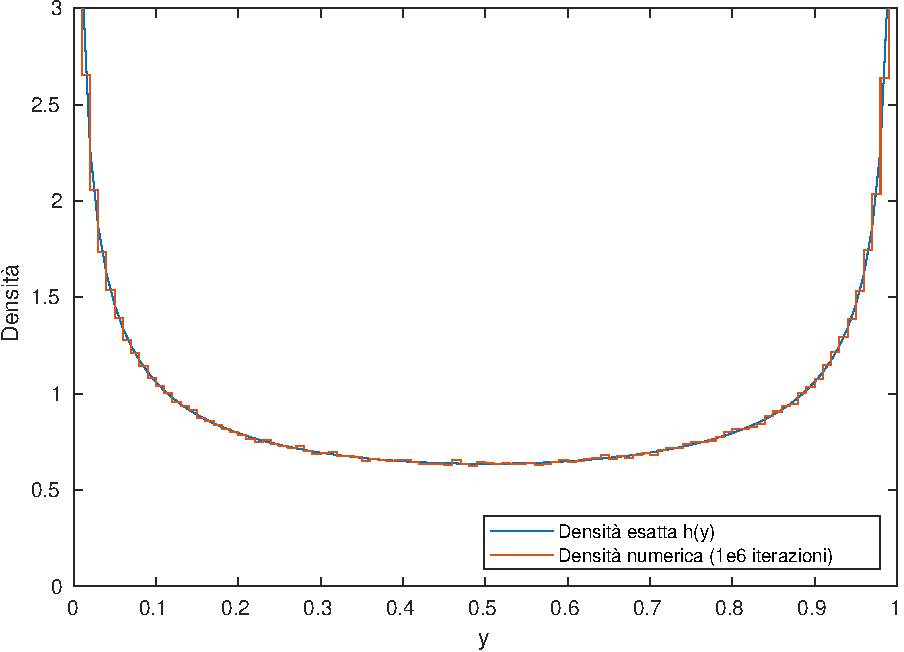
\includegraphics[height=0.4\textheight]{logistic-ergodicity.pdf}
\caption{Confronto tra medie temporali empiriche \eqref{eq:ergodicità-somma}
e media spaziale esatta \eqref{eq:ergodicità-integrale}.}
\label{fig:logistic-ergodicity}
\end{figure}

Per riassumere visivamente le strutture di equilibrio al variare di $a$ in $[0,4]$,
abbiamo scritto il Programma \ref{prog:logistic-bifurcation-diagram} che genera
il \emph{diagramma di biforcazione} dell'equazione logistica,
riportato in Figura \ref{fig:diagramma-di-biforcazione}.
In questo tipo di diagramma, a ogni pixel dell'immagine è associato un
valore di~$a$ (sulle ascisse, da 0 a 4) e un piccolo intervallo attorno
a un valore~$y$ (sulle ordinate, da 0 a 1).
Per generare una colonna dell'immagine (quindi, fissato $\bar{a}$) si sceglie
un valore iniziale $y_0$ e poi si effettuano due simulazioni consecutive
della dinamica: la prima per $N \gg 0$ passi in modo che $y_n$ sia attratto
dalla struttura di equilibrio attiva per $a = \bar{a}$, e la seconda per
altri $M \gg 0$ passi andando a marcare tutti i pixel dell'immagine a cui sono associati
degli intervalli che contengono almeno uno dei punti $y_{N+1},\dots,y_{N+M}$.
In questo modo, la colonna corrispondente a ogni valore di $a$ in un diagramma
di biforcazione fornisce una rappresentazione approssimativa della
struttura di equilibrio dell'equazione logistica $y_{n+1} = a y_n (1-y_n)$.

\lstinputlisting[float=tbp, label=prog:logistic-bifurcation-diagram,
caption={Calcolo del diagramma di biforcazione.}]{logistic_bifurcation_diagram.m}

\begin{figure}[tbp]
\centering
\begin{tikzpicture}[trim axis left, trim axis right]
\begin{axis}[
	enlargelimits=false,
	axis on top,
	xlabel={$a$},
	ylabel={$y$},
	width=0.9\textwidth,
	height=0.6\textwidth,
]
\addplot graphics [
	xmin=0,xmax=4,
	ymin=0,ymax=1,
] {bifurcation-diagram-edited.png};
\end{axis}
\end{tikzpicture}
\caption{Diagramma di biforcazione dell'equazione logistica discreta.}
\label{fig:diagramma-di-biforcazione}
\end{figure}

\begin{figure}[tbp]
\centering
\begin{tikzpicture}[trim axis left, trim axis right]
\begin{axis}[
	enlargelimits=false,
	axis on top,
	xlabel={$a$},
	ylabel={$y$},
	width=0.9\textwidth,
	height=0.9\textwidth,
]
\addplot graphics [
	xmin=3.5,xmax=4,
	ymin=0,ymax=1,
] {bifurcation-diagram-zoomed-edited.png};
\end{axis}
\end{tikzpicture}
\caption{Diagramma di biforcazione dell'equazione logistica discreta (dettaglio).}
\label{fig:diagramma-di-biforcazione-dettaglio}
\end{figure}

Nonostante la risoluzione limitata dell'immagine in Figura
\ref{fig:diagramma-di-biforcazione}, possiamo in effetti riconoscere il fenomeno
di raddoppio del periodo per valori di $a$ compresi tra 3 e 3.57.
Inoltre, l'aspetto della regione a destra di $a = 3.57$ lascia intuire la
complessità del regime caotico. La scelta del valore iniziale $y_0$ non è
particolarmente importante, perché quasi ogni valore viene attratto dalle
stesse strutture di equilibrio;
nella pratica la scelta $y_0 = 1/2$ funziona bene e converge rapidamente,
a parte il caso $a = 4$ in cui è uno dei punti dell'insieme di misura nulla
la cui dinamica non è ergodica (finisce in 0). Nel caso $a = 4$ abbiamo quindi
scelto $y_0 = 1/3$.


















